\section{Introduction}


The rapid adoption of Large Language Model (LLM)
agents across commercial coding tools (e.g., Claude Code, Codex,
OpenCode, and Pi Coding Agent), autonomous research frameworks, and
tool-orchestration systems~\cite{agentbench,swebench,autogen} marks a
fundamental shift in computing, upgrading LLMs from text
generators into autonomous, long-horizon task execution
engines~\cite{react,toolformer,memgpt}. To perform complex workflows
across software development and daily automation, these agents are
granted unprecedented agency, increasing their risk of 
exposure to
potentially untrusted
external content, including live web search results, dynamic local
file trees, API payloads, and Model Context Protocol (MCP) tool
outputs~\cite{mcp,mcpsafetyaudit,mcpfirstglance}.

This autonomy creates a severe security paradox: \emph{The
  very privileges that empower agents to orchestrate environments also
  open broad, untrusted channels for remote exploitation}. Consequently, critical operational pipelines, from memory modules to third-party tool responses, have increasingly been
exploited via prompt injection and data poisoning
attacks~\cite{perez-ribeiro,greshake,liu-injection,tensortrust,injecagent,agentpoison,wan-poisoning}.
Since agents hold system-level execution rights, successful
exploits can yield immediate, devastating impacts on production
environments~\cite{mcpsafetyaudit}. Recent real-world
vulnerabilities have underscored this urgency. For instance,
\texttt{CVE-2025-32711} (EchoLeak) demonstrated how a zero-click,
malicious email could induce Microsoft 365 Copilot to disclose
sensitive user data~\cite{cve202532711,echoleak}, while
\texttt{CVE-2025-53773} and \texttt{CVE-2026-29783} revealed that
malicious repository files and forged MCP responses could hijack
GitHub Copilot to execute arbitrary local
code~\cite{cve202553773,cve202629783}.

% Masked 2026-08-26: trilemma figure parked until a cleaner redraw.
\iffalse
\begin{figure}[!t]
  \centering
  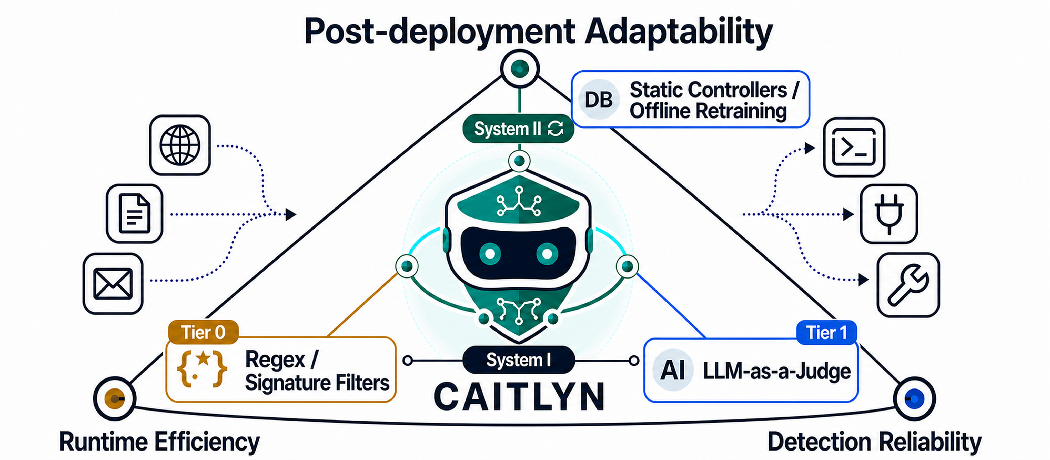
\includegraphics[width=\linewidth]{figures/agent_defense_trilemma_imagegen_v8_aligned.pdf}
  \caption{
    The trilemma of agent defense. Existing defenses tend to prioritize runtime
    efficiency, detection reliability, or post-deployment adaptability,
    whereas CAITLYN targets a balanced operating point across all three
    objectives while mediating agent inputs and tool interactions.
  }
  \label{fig:agent-defense-trilemma}
\end{figure}
\fi


To mitigate these threats, the community has proposed diverse
defenses, yet existing paradigms expose a fundamental impasse that we
call the \emph{trilemma of agent defense}: \textbf{a)} Deterministic
signature and regular-expression
filters~\cite{nemoguardrails,promptguard} deliver \emph{runtime
efficiency} by executing at sub-millisecond speeds with zero token cost,
but they fall victim to trivial adversarial obfuscation or semantic
mutations~\cite{tensortrust,liu-injection}. \textbf{b)} Heavyweight LLM-based
guardians~\cite{zheng-judge} and fine-tuned discriminator
models~\cite{promptguard,protectaideberta} deliver \emph{contextual
precision} through high detection accuracy, yet they burden mostly benign runtime traffic
with substantial inference latency, high token costs, and
persistent false positives on standard user tasks. \textbf{c)} Structural access
controllers (e.g., AgentWard, ClawGuard~\cite{agentward,clawguard})
and offline-retrained models enforce static perimeter boundaries for
\emph{lifelong adaptability}, yet they remain fundamentally incapable
of continuously absorbing evolutionary, post-deployment attack payloads
without time-consuming manual rule authoring or costly offline re-training. In
our view, a practical agent defense system should jointly target
ultra-low overhead, strict false-positive bounds, and seamless
adaptation to novel attack variants, while current point-solution defenses
inevitably collapse along at least one axis of this trilemma.

To reconcile this fundamental trade-off, we propose \textbf{C}ontinuous
\textbf{A}gents for \textbf{I}njection
\textbf{T}hreats via \textbf{L}ifelong \textbf{Y}ielding
\textbf{N}exus (\textbf{CAITLYN}), an agent-agnostic defense middleware that
re-conceptualizes security guards not as static heuristics, but as
executable, self-extending skill libraries. CAITLYN draws inspiration
from Counterexample-Guided Inductive Synthesis
(CEGIS)~\cite{sketch2006,sygus2013,flashfill2011}, a fundamental
engine in program synthesis. Our core operational insight is
that \emph{every adversarial payload bypassing the existing defense
  acts as a concrete counterexample, and every counterexample serves
  as a formal specification to synthesize a more robust defense
  skill.}

Architecturally, CAITLYN separates defense execution into a
dual-system design. \textbf{System~I} serves as
the fast runtime engine, applying a library of pre-verified defense
skills to incoming traffic. \textbf{System~II} operates as a
deliberative, synthesis-driven loop that expands the skill library when
novel attacks emerge. When System~I misses an attack payload or
receives a seed encounter, System~II invokes an LLM-driven generator to
produce candidate defense skills and a deterministic verifier to test
each candidate against an attack corpus (i.e., positive specifications) and
a benign functional dataset (negative constraints). Candidates that
fail acceptance criteria are rejected to guide iterative refinement. A
candidate that passes verification is deployed with traceable lineage,
reducing the need for manual rule engineering.

We instantiate this dual architecture with System~I for runtime
enforcement and System~II for synthesis, seeded with a library of 24
defense skills spanning three categories, curated from an analysis of
the 2024 to 2026 literature. Tier~0, the scripted gatekeeper, executes
rule sets without an LLM call, addressing
the runtime efficiency requirement. Tier~1, the minimal-output
evaluator, performs LLM-based detection through a compact
status-and-score contract, providing contextual coverage while reducing the
latency of full LLM judges. System~II hosts the CEGIS synthesis loop
and behavioral monitor, supporting lifelong adaptability while
enforcing benign specification constraints to limit false positives.

We evaluate CAITLYN across standard agent security
benchmarks~\cite{agentdojo,aspi,safeclawbench} and
\emph{Emerging}, a new delivery-aware benchmark designed to evaluate
post-deployment defense evolution against emerging injection
techniques. On standard benchmarks, CAITLYN matches the detection
performance of state-of-the-art defenses at lower token overhead than
LLM-as-a-judge baselines. On \emph{Emerging}, static baselines and
the initial System~I configuration remain vulnerable. System~{II}
turns these observed failures into counterexamples and autonomously
synthesizes several new deployable defense skills that substantially reduce
attack success across three agent environments, demonstrating the
effectiveness of CAITLYN against unknown attacks.


In summary, our key contributions are as follows:
\begin{itemize}[nosep]
    \item \textbf{Paradigm and Architecture:} We introduce CAITLYN, an
      agent-agnostic defense middleware that treats security rules as
      executable, self-extending skill libraries. By decoupling runtime
      enforcement (System~I) from dynamic skill synthesis (System~II),
      CAITLYN explores the traditional defense trilemma between runtime
      efficiency, detection precision, and post-deployment adaptability.
  \item \textbf{Defense Synthesis:} We present a
  counterexample-guided synthesis mechanism for agent defenses. The
  engine automatically mutates candidate defense skills using an LLM generator and
  validates them through a deterministic verifier against dual
  specifications.
  \item \textbf{Benchmark and Evaluation:} We construct
    \emph{Emerging}, an expert-curated benchmark capturing novel
    injection techniques. Extensive evaluations demonstrate
    that CAITLYN matches state-of-the-art defense quality at
    lower token overhead, while demonstrating autonomous
    adaptation against unfamiliar attack vectors.
\end{itemize}

